\section{Análisis comparativo}

En las secciones anteriores pudimos ver el desempeño de cada filtro por separado, veamos ahora la comparativa utilizando las medidas PESQ y STOI. En la figura \ref{fig:ch8_pesq_comparison} podemos ver la variación media en la PESQ, tanto para el filtro adaptativo como para el filtro neuronal para los distintos niveles de ruidos utilizados.

\begin{figure}[h]
	\centering
	\centerline{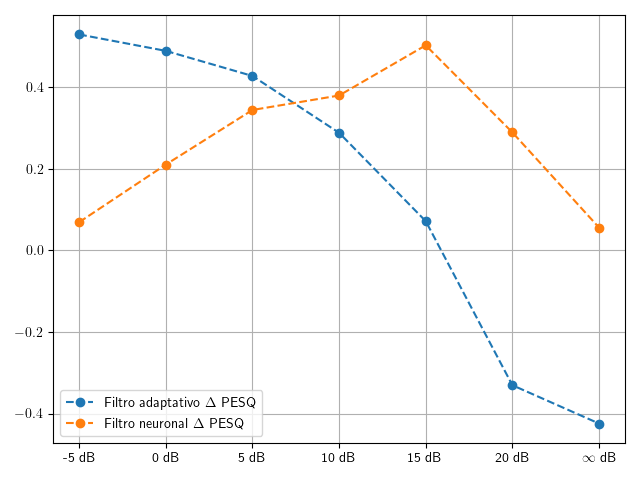
\includegraphics[scale=0.75]{images/ch8/comparison_pesq.png}}
	\caption{Comparación PESQ en función de la SNR.}
	\label{fig:ch8_pesq_comparison}
\end{figure}

Para el caso del filtro adaptativo vemos que el mejor desempeño se obtuvo para un SNR de \SI{-5}{dB} y para SNRs mayores, la variación media disminuyó. La disminución en el desempeño a medida que aumenta la SNR se debe al error en estado estacionario del filtro adaptativo como vimos en la figura \ref{fig:ch6_mse_and_noise_level}.

Por otro lado, el filtro neuronal logra el mejor desempeño para los \SI{15}{dB} y con un valor similar al del caso del filtro adaptativo. A diferencia del filtro adaptativo, tanto para SNRs altos como para bajos el desempeño disminuyó respecto del obtenido para \SI{15}{dB}. La disminución en el desempeño, en bajos niveles de SNR, se debe a los errores de estimación en el espectro y en altos niveles de SNR, al error de generalización de la red, como vimos en la figura \ref{fig:ch7_mse_and_noise_level}.	

En la figura \ref{fig:ch8_stoi_comparison} podemos ver la variación media en la STOI, tanto para el filtro adaptativo como para el filtro neuronal para los distintos niveles de ruidos utilizados.

\begin{figure}
	\centering
	\centerline{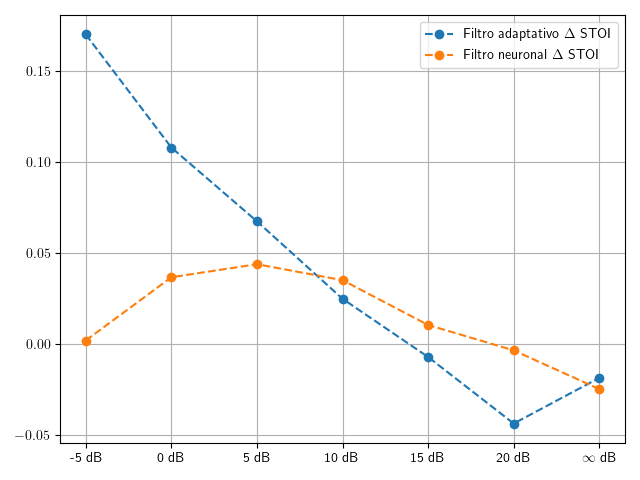
\includegraphics[scale=0.75]{images/ch8/comparison_stoi.png}}
	\caption{Comparación STOI en función de la SNR.}
	\label{fig:ch8_stoi_comparison}
\end{figure}

Para el caso de la STOI se obtuvieron características similares que para la PESQ, es decir, el filtro adaptativo tuvo un mejor desempeño a bajos niveles de SNR y el filtro neuronal se desempeñó mejor que el adaptativo a niveles altos de SNR. A diferencia de la PESQ, en este caso el desempeño del filtro adaptativo a bajos niveles de SNR fue muy superior. La máxima variación en la STOI para el filtro adaptativo es más de 3 veces la máxima variación en la STOI para el filtro neuronal.

También resulta interesante comparar como fue el desempeño de cada tipo de filtro en función del ruido, tanto para la medida PESQ como la medida STOI. En las figuras \ref{fig:ch8_pesq_comparison_by_noise} y \ref{fig:ch8_stoi_comparison_by_noise} podemos ver los resultados obtenidos.

\begin{figure}
	\centering
	\centerline{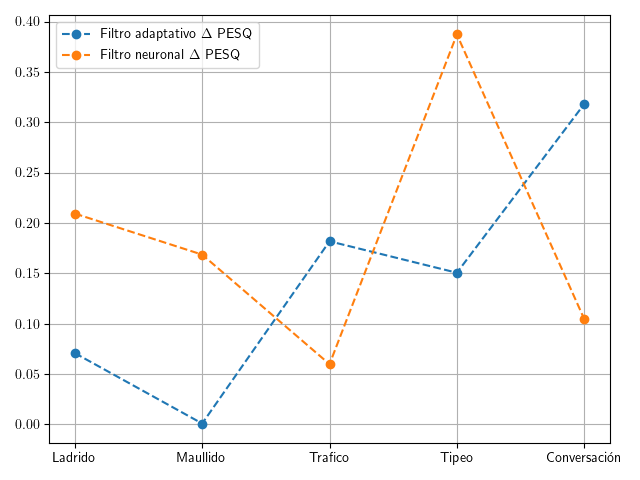
\includegraphics[scale=0.75]{images/ch8/comparison_pesq_by_noise.png}}
	\caption{Comparación PESQ en función del tipo de ruido.}
	\label{fig:ch8_pesq_comparison_by_noise}
\end{figure}

\begin{figure}
	\centering
	\centerline{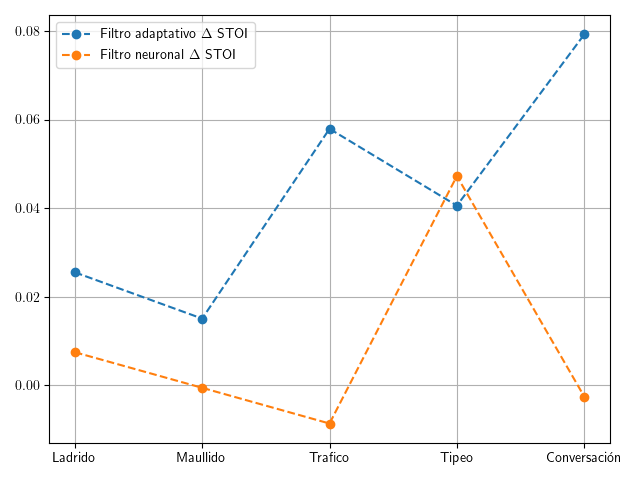
\includegraphics[scale=0.75]{images/ch8/comparison_stoi_by_noise.png}}
	\caption{Comparación STOI en función del tipo de ruido.}
	\label{fig:ch8_stoi_comparison_by_noise}
\end{figure}

En relación a la medida PESQ, se observa en la figura \ref{fig:ch8_pesq_comparison_by_noise}, que el filtro neuronal fue superior en la clases de ruido \emph{Ladrido} y \emph{Maullido}, donde el filtro adaptativo tuvo dificultades. A su vez, los ruidos \emph{Tráfico} y \emph{Conversación}, que fueron mas difíciles de filtrar para la red debido a su complejidad espectral, el filtro adaptativo logró un buen desempeño.

Respecto de la medida STOI, como ya vimos en la sección \ref{sec:resultados_filtro_neuronal}, el filtro neuronal no logró buenos resultados, lo que llevó al filtro adaptativo a ser superior en prácticamente toda las clases de ruido.